\documentclass[11pt,a4paper]{ltjsarticle}
\usepackage[margin=25mm]{geometry}
\usepackage{amsmath,amsthm,enumitem,listings,longtable,booktabs,tikz,float}

\newenvironment{foldnote}{\begin{quote}}{\end{quote}}
\begin{document}
\noindent Start 行間を記す。\par
\vspace*{195mm}
\paragraph{折り目} Runline 白い紙を重ねる。
\section{Folded}
\subsection{Edges}
First 端を揃える。\\Second 裏を見る。\\Third 元に戻す。
\clearpage
\noindent Priorpage 紙。\par\vspace*{216mm}\par\section{Floatmark}
\begin{figure}[htbp]\centering\rule{32mm}{10mm}\caption{Topmark}\end{figure}
\noindent Floatend 紙の位置を記す。\\Secondleaf 紙。
\begin{description}[style=nextline]
\item[短] Shortbody 折り目。
\item[幅広い紙の端] Longbody 裏の印。
\end{description}
\begin{description}[style=nextline,leftmargin=4em,labelwidth=2em,labelsep=.75em]
\item[赤] Redbody 表の印。
\item[長い折り目] Widebody 裏の印。
\end{description}
\noindent Gridstart\par
\noindent 折紙窓札折紙窓札折紙窓札折紙窓札折紙窓札折紙窓札折紙窓札折紙窓札折紙窓札折紙窓札折紙窓札折紙窓札折紙窓札折紙窓札折紙窓札。\par
\noindent 東の「紙窓」、西の「細板」、青の「角札」、赤の「端板」、白の「折板」、奥の「紙窓」、手前の「角札」、南の「折板」。\par
\noindent 紙A紙B紙C紙D紙E紙F紙G紙H紙I紙J紙K紙L紙M紙N紙O紙P紙Q紙R紙S紙T紙U紙V紙W紙X紙Y紙Z紙。\par
\noindent Gridend
\clearpage
\noindent Mathstart 紙。
\[ a = 27 \]
\[ b = 28 \]
\noindent Mathmid 紙。
\begin{align*} c &= 29 \\ d &= 30 \end{align*}
\begin{gather*} e=31 \\ f=32 \end{gather*}
\noindent Mathend 紙。
\begin{proof} Proofstart $x$ の幅を測る。
\[ g=\begin{cases}1 & x>0 \\ 0 & x\le0\end{cases} \]
Proofend 記録する。\end{proof}
\noindent Mixedbefore 紙。\par
\noindent Mixedline {\small 小さな窓}{\Large 大きな窓}。\par
\noindent Mixedafter 紙。% 裏面

{\small Newpara 別の段落。}
\paragraph{札} Runend 端を読む。
\section{Afterrun}
\begin{foldnote}InsideNote 縁を記す。\end{foldnote}
\subsection{Afternote}
\noindent Boxline \fbox{白い札}
\section{Afterbox}
\noindent Versestart 窓。
\begin{verse}Versemid 青い印。\\ 赤い印。\end{verse}
\noindent Verseend 紙。
\clearpage
\noindent Lstart 行。
\begin{lstlisting}[basicstyle=\small\ttfamily,numbers=left,caption={Listcap},frame=single]
a
b
c
d
e
f
g
h
i
j
k
l
m
n
o
p
q
\end{lstlisting}
\noindent Lend 紙。
\begin{longtable}{ll}
\caption{Longcap}\\
\toprule RowA & 北 \\ \midrule RowB & 南 \\ RowC & 西 \\ \bottomrule
\end{longtable}
\noindent LTend 紙。\par\bigskip\noindent\rule{30mm}{1pt}\par
\noindent Ruleend 紙。
\clearpage
\noindent Tabstart 窓。
\begin{table}[H]\centering\begin{tabular}{ll}\toprule TabA & 北 \\ TabB & 南 \\ \bottomrule\end{tabular}\caption{Tabcap}\end{table}
\noindent Tabend 紙。
\section{Fighead}
\begin{figure}[H]\centering
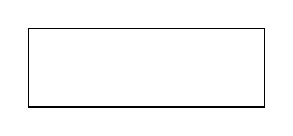
\begin{tikzpicture}\draw (0,0) rectangle (3,1);\end{tikzpicture}
\caption{Figcap}
\end{figure}
\noindent Figend 紙。

\clearpage
\section{Leafverse}
\begin{verse}Verseopen 紙。\\Verseclose 縁。\end{verse}
\noindent Beforeplain 紙。
\begin{lstlisting}[basicstyle=\small\ttfamily,numbers=left,caption={Plaincap}]
width = 1
count = 4
\end{lstlisting}
\noindent Afterplain 紙。
\begin{longtable}{ll}
\caption{Plainlong}\\
PlainA & 北 \\ PlainB & 南 \\
\end{longtable}
\noindent Afterlong 紙。
\section{Figures}
\begin{figure}[htbp]\centering
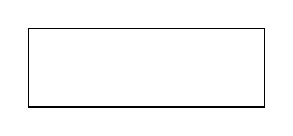
\begin{tikzpicture}\draw (0,0) rectangle (3,1);\end{tikzpicture}
\caption{Herefig}
\end{figure}
\noindent Afterfig 紙。
\end{document}
